\documentclass[11pt]{article}
\title{How the Codynamic Book Machine Works}
\author{Arthur Petron}
\usepackage[margin=1in]{geometry}
\usepackage{graphicx}
\usepackage{amsmath,amssymb,mathtools}
\usepackage{tikz}
\usetikzlibrary{positioning,arrows.meta}
\usepackage{hyperref}
\graphicspath{{media/}{media/diagrams/}{images/}{artwork/}}

\begin{document}

\section*{The Coordination Problem in Long-Form Writing}

Long-form writing fails for a simple reason: the work is not one thing. A book is an evolving collection of outlines, section drafts, claims, citations, figures, editorial notes, and build artifacts, each of which can change at a different pace. When those parts are managed separately, they drift. The outline may promise a structure that the prose no longer follows; a section may introduce a claim that never receives a citation; a diagram may reflect an earlier argument; a review comment may be resolved in one file but remain visible in another; and a successful build may conceal the fact that the manuscript is internally inconsistent.

This drift is especially costly in long-form technical writing, where coherence depends on more than local correctness. A chapter can read well sentence by sentence while still failing at the level of argument, terminology, or dependency order. A definition introduced in one section may be reused elsewhere before it is stabilized. A reference added late in the process may support one paragraph but not the surrounding discussion. A figure can become stale as soon as the surrounding explanation changes. Even the compiled output can lag behind the source of truth if the manuscript is assembled from multiple moving parts without a disciplined coordination model.

The problem is not merely that books are large. It is that they are heterogeneous. The outline expresses intent, the draft expresses prose, the bibliography expresses evidence, the diagram set expresses structure, the review cycle expresses editorial judgment, and the build system expresses what can actually be compiled. If these surfaces are treated as independent, authors and tools must continually reconstruct the relationships among them by hand. That reconstruction is fragile, repetitive, and easy to get wrong.

In conventional workflows, this fragility appears as familiar failure modes. An outline is revised after sections have already been drafted, leaving the manuscript misaligned with the plan. A citation is added in one place but not propagated to related claims. A diagram is requested too early and then forgotten when the argument changes. Review feedback is recorded in comments, but the corresponding text is not updated consistently across files. Build errors are fixed locally without addressing the underlying dependency that caused them. Over time, the manuscript accumulates small inconsistencies that are individually minor but collectively expensive.

The coordination problem, then, is the challenge of keeping all of these surfaces synchronized while the book is still being written. It is not enough to generate text; the system must preserve alignment among intent, structure, evidence, visuals, editorial state, and compiled artifacts. The Codynamic Book Machine is designed around that requirement. Its central claim is that a book can be managed as a living technical object only if the relationships among its parts are made explicit and continuously maintained.

That requirement motivates the rest of this paper. The next section states the thesis of the machine as a codynamic system: one in which outline, agents, task queues, dependencies, artifacts, and compiled outputs evolve together rather than as isolated files. Subsequent sections ground that thesis in the repository itself, showing how the current implementation represents the work, routes tasks, registers references, requests diagrams, and preserves a durable record of the manuscript as it changes.

\begin{figure}[htbp]
\centering
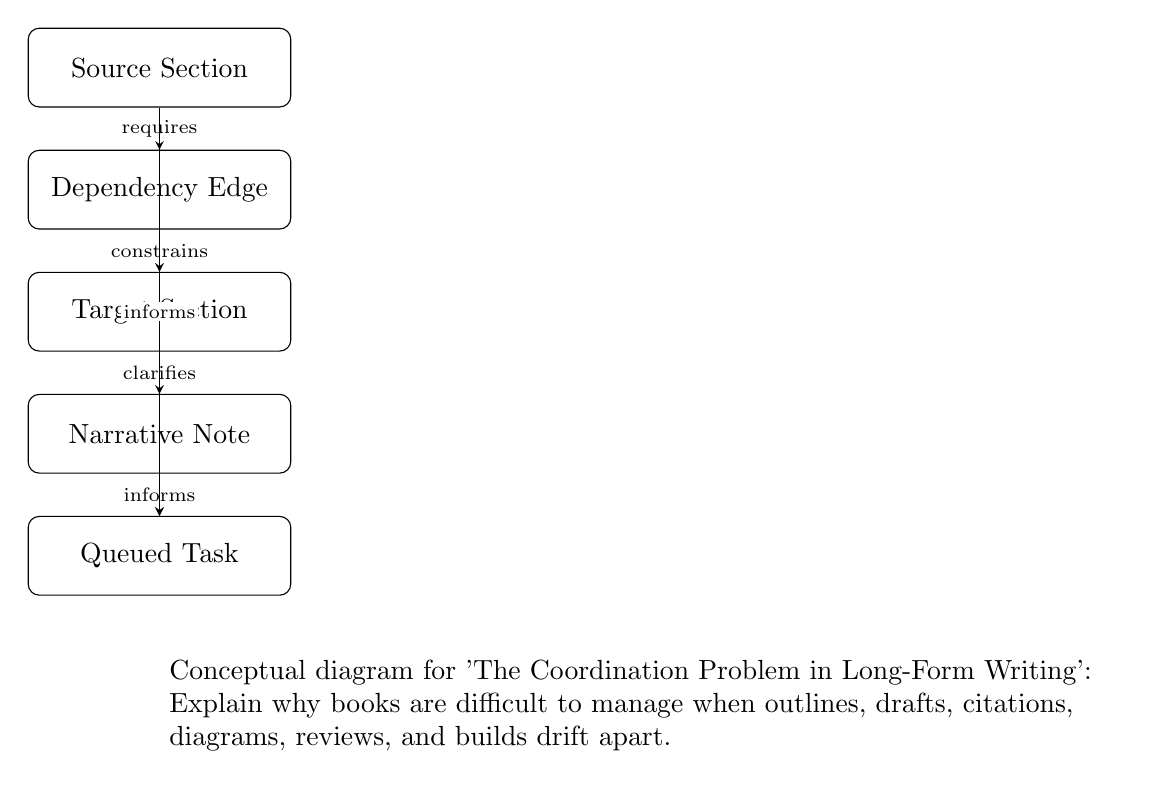
\begin{tikzpicture}[>=stealth, node distance=2.2cm,
  concept/.style={draw, rounded corners, align=center, text width=3.1cm, minimum height=1cm},
  relation/.style={font=\scriptsize, fill=white, inner sep=1pt}]
\node[concept] (n1) at (0,0.0) {Source Section};
\node[concept] (n2) at (0,-1.55) {Dependency Edge};
\node[concept] (n3) at (0,-3.1) {Target Section};
\node[concept] (n4) at (0,-4.65) {Narrative Note};
\node[concept] (n5) at (0,-6.2) {Queued Task};
\draw[->] (n1) -- node[relation] {requires} (n2);
\draw[->] (n2) -- node[relation] {constrains} (n3);
\draw[->] (n3) -- node[relation] {clarifies} (n4);
\draw[->] (n4) -- node[relation] {informs} (n5);
\draw[->] (n1) -- node[relation] {informs} (n5);
\node[align=left, text width=12cm, anchor=north west] at (0,-7.4) {Conceptual diagram for 'The Coordination Problem in Long-Form Writing': Explain why books are difficult to manage when outlines, drafts, citations, diagrams, reviews, and builds drift apart.};
\end{tikzpicture}

\caption{Conceptual diagram for ``The Coordination Problem in Long-Form Writing'': books become difficult to manage when outlines, drafts, citations, diagrams, reviews, and builds drift apart.}
\end{figure}


\end{document}
